\input ../SlidePreamble
\input ../preamble

\newcommand{\solution}[1]{\bigskip {\bf Solution}: #1}

\begin{document}

{\Huge
  \centerline{\bf TTIC 31230, Fundamentals of Deep Learning}
  \bigskip
  \centerline{David McAllester, Winter 2019}
  \vfill
  \centerline{\bf Stochastic Gradient Descent (SGD)}
  \vfill
  \centerline{The Classical Convergence Theorem}
  \vfill
  \centerline{Momentum, RMSProp, and Adam}
  \vfill
  \centerline{Hyperparameter Conjugacy}

\slide{Vanilla SGD}

$$\Phi \;\minuseq\; \eta \hat{g}$$

\vfill
\begin{eqnarray*}
  \hat{g} & = & E_{(x,y) \sim \mathrm{Batch}}\;\nabla_\Phi\;\mathrm{loss}(\Phi,x,y) \\
  \\
  \\
  g & = & E_{(x,y) \sim \mathrm{Pop}}\;\nabla_\Phi\;\mathrm{loss}(\Phi,x,y) \\
\end{eqnarray*}

\slide{Issues}

\vfill
\begin{itemize}
\item {\bf Gradient Estimation.} The accuracy of $\hat{g}$ as an estimate of $g$.

  \vfill
\item {\bf Gradient Drift (second order structure).} The fact that $g$ changes as the parameters change.

  \vfill
\item {\bf Convergence.} To converge to a local optimum the learning rate must be gradually reduced toward zero.

  \vfill
  \item {\bf Exploration.} Since deep models are non-convex we need to search over the parameter space.  SGD can behave like MCMC.
\end{itemize}

\slide{A One Dimensional Example}

Suppose that $y$ is a scalar, and consider

\begin{eqnarray*}
 \mathrm{loss}(\beta,y) & = & \frac{1}{2}(\beta - y)^2 \\
 \\
  g & = &  \nabla_\beta\;E_{y \sim \mathrm{Pop}}\;\frac{1}{2}(\beta - y)^2 \\
  \\
  & = & \beta - E_{y \sim \mathrm{Pop}} \; y \\
  \\
  \hat{g} & = &\beta - E_{y \sim \mathrm{Batch}} \;y
\end{eqnarray*}

\vfill
Even if $\beta$ is optimal, for a finite batch we will have $\hat{g} \not = 0$.

\slide{The Classical Convergence Theorem}

$$\Phi \;\minuseq \; \eta_t \nabla_\Phi\;\mathrm{loss}(\Phi,x_t,y_t)$$

\vfill
For ``sufficiently smooth'' non-negative loss with

\vfill
$$\eta_t > 0\;\;\;\;\mbox{and}\;\;\;\;\lim_{t \rightarrow \infty} \;\eta_t = 0\;\;\;\;\mbox{and}\;\;\;\;\sum_t \eta_t = \infty,$$

\vfill
we have that the training loss of $\Phi$ converges (in practice $\Phi$ converges to a local optimum of training loss).

\vfill
{\Large
\vfill
{\bf Rigor Police:} One can construct cases where $\Phi$ diverges to infinity, converges to a saddle point, or even converges to a limit cycle.

\vfill
{\bf Rigor Police:} This theorem is usually stated with an additional condition that $\sum_t \;\eta_t^2 < \infty$.  I believe that this additional condition is not required.

}

\slide{Physicist's Proof of the Convergence Theorem}

Since $\lim_{t \rightarrow 0} \;\eta_t = 0$ we will eventually get to arbitrarilly small learning rates.

\vfill
For sufficiently small learning rates any meaningful update of the parameters will be based on an arbitrarily large sample
of gradients at essentially the same parameter value.

\vfill
An arbitrarily large sample will become arbitrarily accurate as an estimate of the full gradient.

\vfill
But since $\sum_t \eta_t = \infty$, no matter how small the learning rate gets, we still can make arbitrarily large motions in parameter space.

\slidetwo{SGD as a form of MCMC}{Learning Rate as a Temperature Parameter}

\centerline{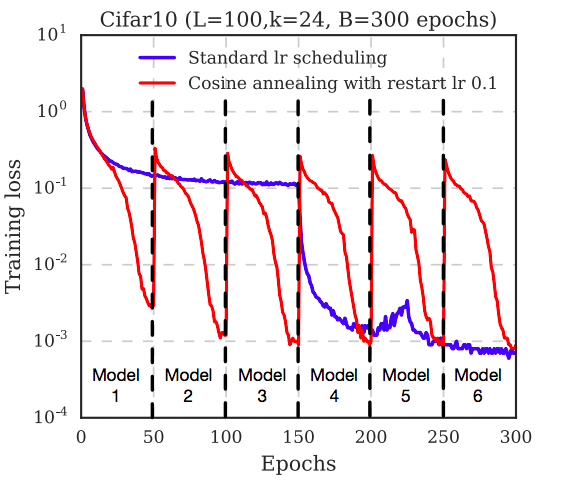
\includegraphics[height= 4in]{../images/AnnealingSGD}}
\centerline{\Large Gao Huang et. al., ICLR 2017}

\slide{}
\centerline{\bf Standard Non-Vanilla SGD Algorithms}
\vfill
\vfill

\slideplain{Digression on Running Averages}
Consider a sequence $x_1$, $x_2$, $x_3$, $\ldots$.
\vfill
For $t \geq N$, consider the average of the $N$ most recent values.
$$\tilde{\mu} = \frac{1}{N} \sum_{s=t-N+1}^t x_s$$

\vfill
This can be approximated more efficiently with
\begin{eqnarray*}
\hat{\mu}_0 & = & 0 \\
\\
\hat{\mu}_t & = & \left(1-\frac{1}{N}\right)\hat{\mu}_{t-1} + \left(\frac{1}{N}\right)x_t\;\;\;t \geq 1 \\
\\
\hat{\mu}_t & \approx & \tilde{\mu}_t \;\;\; t >N
\end{eqnarray*}

\slide{Running Averages}

More explicitly, for $\hat{\mu}_0 = 0$, the update

$$\hat{\mu}_t = \left(1-\frac{1}{N}\right)\hat{\mu}_{t-1} + \left(\frac{1}{N}\right)x_t$$

\vfill
gives

$$\hat{\mu}_t = \frac{1}{N} \sum_{1 \leq s \leq t} \left(1-\frac{1}{N}\right)^{t-s} x_s$$

\vfill
where we have

$$\sum_{n\geq 0} \left(1-\frac{1}{N}\right)^{-n} = N$$

\slide{Momentum}

\begin{eqnarray*}
  {\color{red} v_t} & {\color{red} =} & {\color{red} \left(1-\frac{1}{N_g}\right) v_{t-1} + \eta * \hat{g}_t} \;\;\;\mbox{$N_g$ is typically 10 or 100}\\
  \\
  {\color{red} \Phi_{t+1}} & {\color{red} =} & {\color{red} \Phi_t -  v_t} \\
\end{eqnarray*}

The theory of momentum is generally given in terms of second order structure.


\centerline{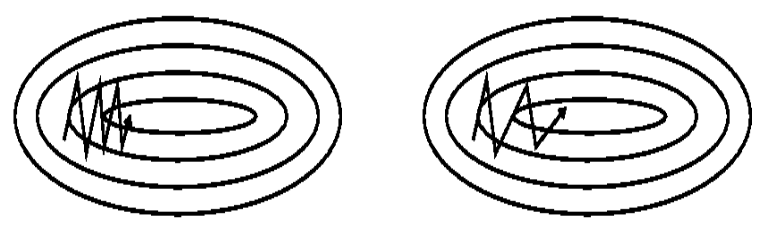
\includegraphics[width = 4in]{../images/momentum}}
\centerline{\Large Rudin's blog}

\slideplain{Momentum}

However, second order analyses are controversial in Deep Learning.

\vfill
We can perhaps get insight by reparameterizing the momentum equations.

\slide{We are Entering a Twilight Zone (TZ)}

\centerline{
\includegraphics[width = 6in]{../images/Twilight}}

\vfill
The twilight zone is material for which I do not know of a reference. 

\slide{Conjugacy of SGD Hyperparameters}

For an objective function $f(x,y)$ we say that $x$ and $y$ are conjugate if changing $x$ does effect the loss gradient for $y$.

\vfill
In other words if

{\color{red} $$\frac{\partial f(x,y)}{\partial x \partial y} = 0$$}

\vfill
We are seeking a nonlinear transformation on hyperparameters yielding robust conjugacy.

\slide{Solving for $\eta$ in terms of $N_g$ (TZ)}

Let $\eta'$ be a learning rate that is appropriate without momentum ($N_g = 1$).

\vfill
We will solve for a learning rate $\eta$ as a function of $N_g$ so as to minimize the perturbation of SGD
as we increase $N_g$.

\slide{An Equivalent Formulation of Momentum}

\begin{eqnarray*}
{\color{red} v_t} & = & \left(1-\frac{1}{N_g}\right) v_{t-1} + \eta \hat{g}_t \\
\\
& = & \left(1-\frac{1}{N_g}\right) v_{t-1} + \frac{1}{N_g}({\color{red} N_g\eta \hat{g}_t}) \\
\\
{\color{red} v_t} & = & {\color{red} N_g\eta\mu_t}\;\;\mbox{for}\;{\color{red} \mu_t = \left(1-\frac{1}{N_g}\right)\mu_{t-1} + \frac{1}{N_g} \hat{g}_t} \\
\\
\Phi_{t+1} & = & \Phi_t - v_t \\
\\
{\color{red} \Phi_{t+1}} & {\color{red} =} & {\color{red} \Phi_t - N_g\eta\mu_t} 
\end{eqnarray*}

\slide{Solving for $\eta$ (TZ)}

\begin{eqnarray*}
\mu_t & = &  \left(1-\frac{1}{N_g}\right)\mu_{t-1} + \frac{1}{N_g} \hat{g}_t \\
\\
\mbox{we have}\;\Phi_{t+1}& = & {\color{red} \Phi_t - N_g\eta\;\mu_t} \\
\\
\mbox{unperturbed is}\;\Phi_{t+1}& = & {\color{red} \Phi_t - \eta'\mu_t}
\end{eqnarray*}

\vfill
This gives {\color{red} $\eta = \eta'/N_g$}.

\vfill
We expect that that $\eta'$ and $N_g$ exhibit more independence (conjugacy) than $\eta$, $N_g$.

\slide{Scaling $\eta$ and $N_g$ with Batch Size}

Recent work has show that scaling hyper-parameters with the batch size can lead to effective learning with very large (highly parallel)
batches.

\vfill
{\bf Accurate, Large Minibatch SGD: Training ImageNet in 1 Hour}, Goyal et al., 2017.

\vfill
{\bf Don't Decay the Learning Rate, Increase the Batch Size}, Smith et al., 2018


\slide{Solving for $\eta$ as a Function of $B$}

Let $\eta'$ be a learning rate appropriate for $N_g = 1$ and $B = 1$.

\vfill
We will solve for $\eta$ as a function of $\eta'$ and $B$ so as to minimize the perturbation of SGD as we increase $B$.

\slide{Solving for $\eta$ as a function of $B$}

Consider two consecutive updates for a batch size of 1 with learning rate $\eta'$.

\begin{eqnarray*}
  \Phi_{t+1} & = & \Phi_t - \eta' \nabla_\Phi \mathrm{loss}(\Phi_t,x_t,y_t) \\
  \\
  \Phi_{t+2} & = & \Phi_{t+1} - \eta' \nabla_\Phi \mathrm{loss}({\color{red} \Phi_{t+1}},x_{t+1},y_{t+1}) \\\
  \\
  & \approx & \Phi_{t+1} - \eta' \nabla_\Phi \mathrm{loss}({\color{red} \Phi_t},x_{t+1},y_{t+1}) \\
  \\
  & = & \Phi_t - \eta'((\nabla_\Phi \mathrm{loss}(\Phi_t,x_t,y_t)) + (\nabla_\Phi \mathrm{loss}(\Phi_t,x_{t+1},y_{t+1})))
\end{eqnarray*}

\slide{Solving for $\eta$ as a function of $B$}

Let $\eta$ be the learning rate for batch size $B$.

\vfill
\begin{eqnarray*}
  \Phi_{t+2} & \approx & \Phi_t - \eta'((\nabla_\Phi \mathrm{loss}(\Phi_t,x_t,y_t)) + (\nabla_\Phi \mathrm{loss}(\Phi_t,x_{t+1},y_{t+1}))) \\
  \\
  & = & \Phi_t - 2\eta'\;\hat{g}\;\;\;\mathrm{for}\;\;B=2
\end{eqnarray*}

\vfill
We have {\color{red} $\Phi \;\minuseq \; \eta\;\hat{g}$}

\vfill
unperturbed is {\color{red} $\Phi \;\minuseq \; B\eta'\;\hat{g}$}

\vfill
This gives {\color{red} $\eta = B \eta'$}.

\vfill
We expect conjugacy for the parameters $\eta'$ and $B$.

\slide{Solving for $N_g$ as a Function of $B$}

Let $N'_g$ be a momentum parameter appropriate for $B=1$.

\vfill
We will solve for $N_g$ as a function of $B$ so as to minimize the perturbation of SGD as we increase $B$.

\vfill
For batch size $B$, $\hat{\mu}_t$ is an average of $\hat{g}$ over $N_gB$ gradient values.

\vfill
SGD seems minimally perturbed by
$$N_gB = N'_g\;\;\;\mbox{or}\;\;\;{\color{red} N_g = N'_g/B}$$

\vfill
We expect conjugacy for the parameters $N'_g$ and $B$.

\slide{Putting It Together (TZ)}

{\color{red}
\begin{eqnarray*}
N_g & = & \min(1,N'_g/B) \\
\\
\eta & = & B\eta'/N_g
\end{eqnarray*}
}

\vfill
We expect conjugacy for $\eta'$, $N'_g$ and $B$.

\slide{RMSProp}

RMSProp is based on a running average of $\hat{g}[i]^2$ for each real-valued model parameter $i$.

\begin{eqnarray*}
{\color{red} s_t[i]} & {\color{red} =} & {\color{red} \left(1-\frac{1}{N_s}\right) s_{t-1}[i] + \frac{1}{N_s} \hat{g}_t[i]^2}\;\;\;\mbox{$N_s$ typically 100 or 1000} \\
\\
{\color{red} \Phi_{t+1}[i]} & {\color{red} =} & {\color{red} \Phi_t[i] - \frac{\eta}{\sqrt{s_t[i] + \epsilon}}\;\; \hat{g}_t[i]}
\end{eqnarray*}


\slide{RMSProp}
\begin{eqnarray*}
{\color{red} s_t[i]} & {\color{red} =} & {\color{red} \left(1-\frac{1}{N_s}\right) s_{t-1}[i] + \frac{1}{N_s} \hat{g}_t[i]^2}\;\;\;\mbox{$N_s$ typically 100 or 1000} \\
\\
{\color{red} \Phi_{t+1}[i]} & {\color{red} =} & {\color{red} \Phi_t[i] - \frac{\eta}{\sqrt{s_t[i] + \epsilon}}\;\; \hat{g}_t[i]}
\end{eqnarray*}

\vfill
For $B = 1$ we have $s[i] \approx E\;\hat{g}[i]^2  =  g[i]^2 + \sigma[i]^2$

\vfill
We should expect $\sigma[i] >> g[i]$.

\vfill
We can therefore think of RMSProp as {\color{red} $\Phi[i] \;\minuseq\; \eta(\hat{g}[i]/\sigma[i])$}

\slide{RMSProp is Theoretically Mysterious}

{\color{red} $$\Phi[i] \;\minuseq \; \eta\;\frac{\hat{g}[i]}{\sigma[i]}\;\;(1)\hspace{5em}\Phi[i] \;\minuseq \; \eta\;\frac{\hat{g}[i]}{\sigma^2[i]}\;\;(2)$$}

\vfill
Although (1) seems to work better, (2) is better motivated theoretically.  To see this we can consider units.

\vfill
If parameters have units of ``weight'', and loss is in bits, then (2) type checks with $\eta$ having units of bits --- the numerical value of $\eta$
has no dependence on the choice of the weight unit.

\vfill
Consistent with the dimensional analysis, many theoretical analyses support (2) over (1) contrary to apparent empirical performance.

\slide{Scaling $\eta$ with Batch Size for RMSProp (TZ)}

Current RMSProp framework implementations do not scale well with batch size.

\vfill
The meaning of  $\hat{g}_i^2$ changes when increasing $B$.

\vfill
$\hat{g}_i$ is an average over a batch --- averaging reduces variance.

\begin{eqnarray*}
{\color{red} E\; \hat{g}_i^2} & {\color{red} =} & {\color{red} = \; \mu_i^2 + \frac{\sigma_i^2}{B}}
\end{eqnarray*}


\slide{Scaling $\eta$ with Batch Size for RMSProp (TZ)}

\begin{eqnarray*}
{\color{red} E\; \hat{g}_i^2} & {\color{red} = } &{\color{red} \mu_i^2 + \frac{\sigma_i^2}{B}}
\end{eqnarray*}

\vfill
To preserve the behavior of RMSProp while increasing $B$ we need a running average of $g_{b,i}^2$ for individual batch elements $b$.

\vfill
This requires augmenting backpropagation to compute an average (or sum) of $g_{b,i}^2$ as well as an average of
$g_{b,i}$ within each batch.

\slide{Adam --- Adaptive Momentum}

Adam combines momentum and RMSProp.

\vfill
It also uses ``bias correction'' of running averages.

\slide{A Digression on Bias Correction of Running Averages}

Consider a sequence $x_1,\;x_2,\;x_3,\ldots$ and consider the following for $N$ large.

\begin{eqnarray*}
\hat{\mu}_0 & = & 0 \\
\\
\hat{\mu}_t & = & \left(1-\frac{1}{N}\right)\hat{\mu}_{t-1} + \left(\frac{1}{N}\right)x_t
\end{eqnarray*}

\vfill
For $\mu \doteq E\;x$ we have $E\;\hat{\mu}_1 = \mu/N$.

\vfill
For $t << N$ we have $E\;\hat{\mu}_t \approx (t/N)\mu$.

\slide{Bias Correction of Running Averages}

The following running average maintains the invariant that $\hat{\mu}_t$ is exactly the average of $x_1,\ldots,x_t$.

\begin{eqnarray*}
\hat{\mu}_0 & = & 0 \\
\\
\hat{\mu}_t & = & \left(\frac{t-1}{t}\right)\hat{\mu}_{t-1} + \left(\frac{1}{t}\right)x_t \\
\\
\\
& = & \left(1-\frac{1}{t}\right)\hat{\mu}_{t-1} + \left(\frac{1}{t}\right)x_t
\end{eqnarray*}

\vfill
But this fails to track a moving average for $t >> N$.

\slide{Bias Correction of Running Averages}

The following avoids the initial bias toward zero while still tracking a moving average.

\begin{eqnarray*}
\hat{\mu}_0 & = & 0 \\
\\
\hat{\mu}_t & = & \left(1-\frac{1}{\min(N,t)}\right)\hat{\mu}_{t-1} + \left(\frac{1}{\min(N,t)}\right)x_t
\end{eqnarray*}

\vfill
The published version of Adam has a more obscure form of bias correction which yields essentially the same effect.

\slide{Adam (simplified)}

\begin{eqnarray*}
  \mu_0[i] & = & s_0[i] = 0 \\
  \\
  \mu_{t}[i] & = & \left(1-\frac{1}{\min(t,N_g)}\right)\mu_{t-1}[i] + \frac{1}{\min(t,N_g)} \hat{g}_t[i] \\
  \\
  s_{t}[i] & = & \left(1-\frac{1}{\min(t,N_s)}\right)s_{t-1}[i] + \frac{1}{\min(t,N_s)} \hat{g}_t[i]^2 \\
  \\
\Phi_{t+1}[i] & =  & \Phi_t - \frac{\eta}{\sqrt{s_{t}[i] + \epsilon}}\;\;\mu_{t}[i]
\end{eqnarray*}
\slide{END}

} \end{document}

